\subsubsection{Set 1 - Greenyard Maaseik}
\label{sec:PL3_Greenyard1}
%TODO: tekst aanpassen
De opslag- en receptiestatistieken worden weergeven in figuur \ref{fig:PL3ServeMaaseik1}. Bij de opslag komt het teken \# overeen met 0, + en / met 1, ! met 2, - en = met 3.
Jolan Cox heeft volgens de AI één opslag meer gegeven dan volgens de manuele invoer. De foutieve opslag van Hampus Ekstrand is wel door beide genoteerd. Opvallend bij deze vergelijking is dat de manuele invoer positiever is bij verschillende opslagen dan de AI.

De beoordeling van de receptie is op een andere wijze gedaan dan bij de manuele invoer. Bij de manuele invoer wordt er gebruik gemaakt van tekens, terwijl bij de AI-invoer gebruik wordt gemaakt van cijfers. Bij de receptie komt het teken \# overeen met 3, + en / met 2, ! met 1, - en = met 0.
Opmerkelijk is dat Thomas Neyens geen receptie heeft gekregen van de AI, terwijl hij er volgens de manuele invoer wel twee keer receptie heeft genomen. Ook Landon Douglas Currie heeft door AI één receptie minder gekregen dan bij de manuele invoer. Hampus Ekstrand daarentegen heeft dan weer een receptie meer gekregen door de AI. Bij hem is er ook eentje niet beoordeeld kunnen worden. Over het algemeen is de beoordeling tussen de 2 methodes ongeveer gelijk.

\begin{figure}[ht]
\centering
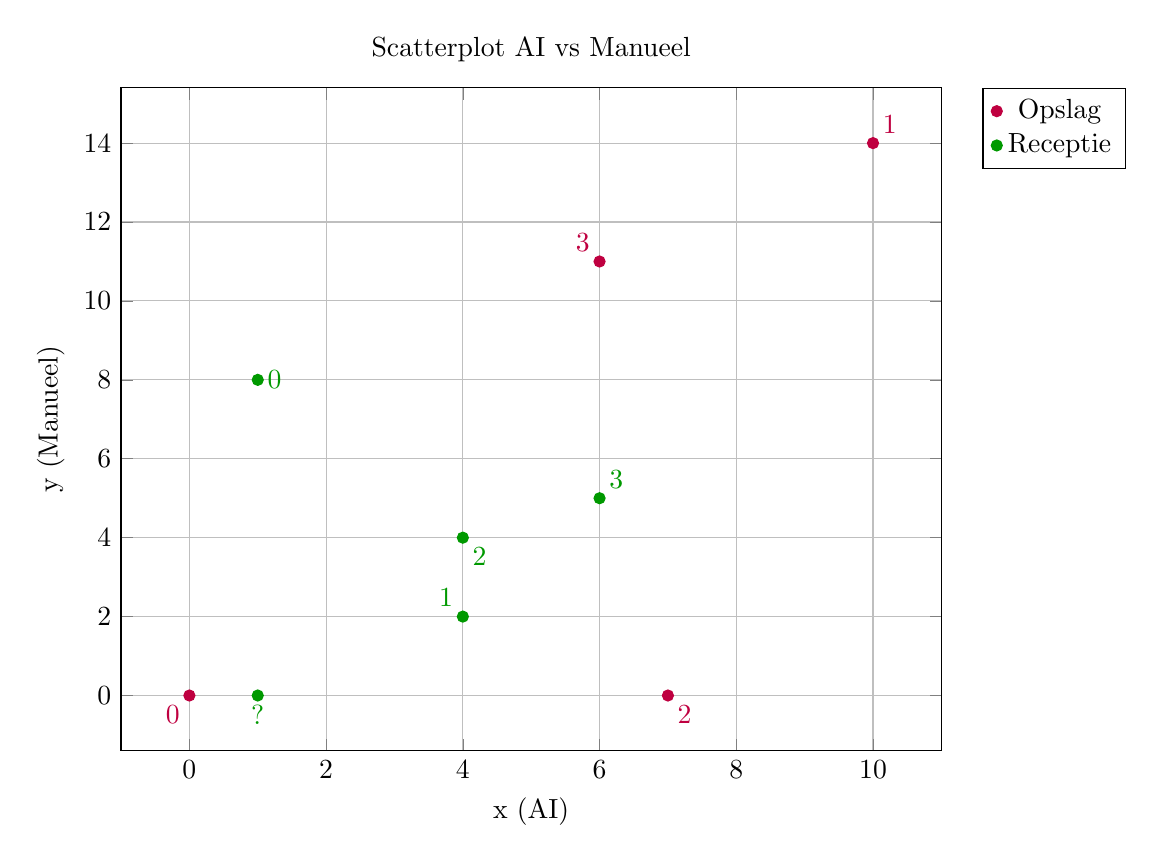
\begin{tikzpicture}
  \begin{axis}[
    title={Scatterplot AI vs Manueel},
    xlabel={x (AI)},
    ylabel={y (Manueel)},
    grid=major,
    legend style={at={(1.05,1)}, anchor=north west},
    width=12cm,
    height=10cm,
    enlargelimits=0.1,
  ]

  % Opslag
  \addplot[
    only marks,
    mark=*,
    color=purple,
  ] table {
    x y
    0 0
    10 14
    7 0
    6 11
  };
  \addlegendentry{Opslag}

  % Labels opslag
  \node at (axis cs:0,0) [anchor=north east, purple] {0};
  \node at (axis cs:10,14) [anchor=south west, purple] {1};
  \node at (axis cs:7,0) [anchor=north west, purple] {2};
  \node at (axis cs:6,11) [anchor=south east, purple] {3};

  % Receptie
  \addplot[
    only marks,
    mark=*,
    color=green!60!black,
  ] table {
    x y
    6 5
    4 4
    4 2
    1 8
    1 0
  };
  \addlegendentry{Receptie}

  % Labels receptie
  \node at (axis cs:6,5) [anchor=south west, green!60!black] {3};
  \node at (axis cs:4,4) [anchor=north west, green!60!black] {2};
  \node at (axis cs:4,2) [anchor=south east, green!60!black] {1};
  \node at (axis cs:1,8) [anchor=west, green!60!black] {0};
  \node at (axis cs:1,0) [anchor=north, green!60!black] {?};

  \end{axis}
\end{tikzpicture}
\caption{AI invoer versus manuele invoer, ingedeeld in opslag en receptie, voor Greenyard Maaseik in set 1.}
\label{fig:PL3ServeMaaseik1}
\end{figure}

Bij de spelverdelingsstatistieken (door Balltime AI in tabel \ref{tab:PL3SetDigMaaseikAI1}) zijn er bepaalde spelers die een andere hoeveelheid hebben. Sommige hebben één minder, andere dan weer één meer dan bij de manuele invoer, tabel \ref{tab:PL3SetMaaseikMan1}.

Bij de verdedigingsstatistieken (door Balltime AI in tabel \ref{tab:PL3SetDigMaaseikAI1}) zijn er twee speler die volgens de AI wel er verdedinngsactie hebben ondernomen, maar bij de manuele invoer niet. Landon Douglas Currie heeft volgens de AI dan weer één verdeding minder dan bij de manuele invoer, zie tabel \ref{tab:PL3DigMaaseikMan1}.

\begin{table}[ht!]
    \centering
    \scriptsize
    \begin{tabular}{|l|c|c|c|c|c|c|c|c|c|} \hline
        \textbf{Speler} & *E\% & Tot & = & / & - & ! & + & \# \\ \hline
        Jolan Cox & 100\% & 2 &  &  &  &  & 2 &  \\ 
        Dawid Pawlun & 88\% & 17 &  & 1 &  &  & 11 & 5 \\ 
        Miquel Angel Fornés & 100\% & 1 &  &  &  &  & 1 &  \\ 
        Hampus Ekstrand & 100\% & 3 &  &  &  &  & 3 &  \\ \hline
    \end{tabular}
    \caption[Manueel ingevoerde spelverdelingsstatistieken voor Greenyard Maaseik in set 1]{\label{tab:PL3SetMaaseikMan1}Manueel ingevoerde spelverdelingsstatistieken voor Greenyard Maaseik in set 1.}
\end{table}

\begin{table}[ht!]
    \centering
    \scriptsize
    \begin{tabular}{|l|c|c|c|c|c|c|c|c|c|} \hline
        \textbf{Speler} & *E\% & Tot & = & / & - & ! & + & \# \\ \hline
        Jolan Cox & 100\% & 1 &  & 1 &  &  &  & \\
        Landon Douglas Currie & 25\% & 4 & 2 &  & 1 &  & 1 & \\ 
        Dawid Pawlun & 100\% & 1 &  &  &  &  & 1 & \\
        Pierre Perin & 0\% & 2 &  &  & 2 &  &  &  \\ \hline
    \end{tabular}
    \caption[Manueel ingevoerde verdedigingsstatistieken voor Greenyard Maaseik in set 1]{\label{tab:PL3DigMaaseikMan1}Manueel ingevoerde verdedigingsstatistieken voor Greenyard Maaseik in set 1.}
\end{table}

\begin{table}[ht!]
  \centering
  \scriptsize
  \begin{tabular}{|l|c|c|c|c|c|c|c|} \hline
    \textbf{Speler} & Ast & TA & SE & PCT & DS & DE \\ \hline
    Jolan Cox & 1 & 2 &  & 50\% & 1 & 0 \\
    Landon Douglas Currie &  &  &   &   & 3 &   \\
    Dawid Pawlun & 9 & 16 &  & 60\% & 1 & 0 \\
    Miquel Angel Fornés & 1 & 2 & & 50\% & 1 & 1 \\
    Hampus Ekstrand &  & 2 &  & 0\% & 1 & \\
    Pierre Perin &   &   &   &   & 2 &   \\ \hline
  \end{tabular}
  \caption[Spelverdelings- en verdedigingsstatistieken gemaakt door Balltime AI voor Greenyard Maaseik in set 1]{\label{tab:PL3SetDigMaaseikAI1}Spelverdelings- en verdedigingsstatistieken gemaakt door Balltime AI voor Greenyard Maaseik in set 1.}
\end{table}

Bij de aanvalsstatistieken (door Balltime AI in tabel \ref{tab:PL3AttBlockMaaseikAI1} en manuele invoer in tabel \ref{tab:PL3AttMaaseikMan1}) is er bij één speler een verschillend aantal aanvallen geregistreed. Pierre Perin heeft volgens de AI één keer minder aangevallen dan bij de manuele invoer. Bij de andere spelers is het aantal bij beide hetzelfde. Ook bij deze set zijn de blokstatistieken door de AI, tabel \ref{tab:PL3AttBlockMaaseikAI1}, niet representatief tegen over de manuele invoer, tabel \ref{tab:PL3BlockMaaseikMan1}.

\begin{table}[ht!]
    \centering
    \scriptsize
    \begin{tabular}{|l|c|c|c|c|c|c|c|c|c|} \hline
        \textbf{Speler} & *E\% & Tot & = & / & - & ! & + & \# \\ \hline
        Samuel Fafchamps & 0\% & 2 &  & 1 &  &  &  & 1 \\ 
        Jolan Cox & 20\% & 5 & 1 & 1 &  &  &  & 3 \\ 
        Miquel Angel Fornés & 100\% & 2 &  &  &  &  &  & 2 \\ 
        Hampus Ekstrand & 0\% & 2 &  & 1 &  &  &  & 1 \\ 
        Pierre Perin & 33\% & 12 &  & 2 &  & 2 & 2 & 6 \\ \hline
    \end{tabular}
    \caption[Manueel ingevoerde aanvalsstatistieken voor Greenyard Maaseik in set 1]{\label{tab:PL3AttMaaseikMan1}Manueel ingevoerde aanvalsstatistieken voor Greenyard Maaseik in set 1.}
\end{table}

\begin{table}[ht!]
    \centering
    \scriptsize
    \begin{tabular}{|l|c|c|c|c|c|c|c|c|c|} \hline
        \textbf{Speler} & *E\% & Tot & = & / & - & ! & + & \# \\ \hline
        Samuel Fafchamps & -100\% & 2 & 2 &  &  &  &  & \\ 
        Dawid Pawlun & -20\% & 5 & 1 & 1 & 2 & & & 1 \\ 
        Miquel Angel Fornés & -20\% & 5 & 1 & 1 &  & 2 & & 1 \\
        Pierre Perin & 0\% & 1 &  &  & 1 &  &  &\\ \hline
    \end{tabular}
    \caption[Manueel ingevoerde blokstatistieken voor Greenyard Maaseik in set 1]{\label{tab:PL3BlockMaaseikMan1}Manueel ingevoerde blokstatistieken voor Greenyard Maaseik in set 1.}
\end{table}

\begin{table}[ht!]
  \centering
  \scriptsize
    \begin{tabular}{|l|c|c|c|c|c|c|c|c|c|c|c|} \hline
    \textbf{Speler} & K & E & TA & Atk\% & Kill\% & Error\% & BS & BA & BE \\ \hline
    Samuel Fafchamps & 1 & 1 & 2 & 0.00 & 50\% & 50\% &  &  &  \\
    Jolan Cox & 3 & 2 & 5 & 0.20 & 60\% & 40\% &   &  &  \\
    Dawid Pawlun &   &   &   &   &   &   & 1 & 1 & \\
    Miquel Angel Fornés & 2 &  & 2 & 1.00 & 100\% & 0\% & 1 & 2 & \\
    Hampus Ekstrand & 2 &  & 2 & 1.00 & 100\% & 0\% &  & & \\
    Pierre Perin & 5 & 2 & 11 & 0.27 & 45\% & 18\% & 0 & 1 & \\ \hline
  \end{tabular}
  \caption[Aanvals- en blokstatistieken gemaakt door Balltime AI voor Greenyard Maaseik in set 1]{\label{tab:PL3AttBlockMaaseikAI1}Aanvals- en blokstatistieken gemaakt door Balltime AI voor Greenyard Maaseik in set 1.}
\end{table}
